\section{项目流程设计}
\subsection{调研部分}
\begin{enumerate}
    \item 对社区居民、居委会负责人、社区医院共20名负责人进行访谈
    \item 设计知识、信念、行为三维度的问卷题目
    \item 发放问卷,回收分析,撰写统计报告。
\end{enumerate}
\subsection{干预部分}
\begin{enumerate}
\item 招募实验人员
\item 进行随机化分组
\item 进行实验
\item 整理数据,分析结果
\end{enumerate};
\begin{figure}[th]
	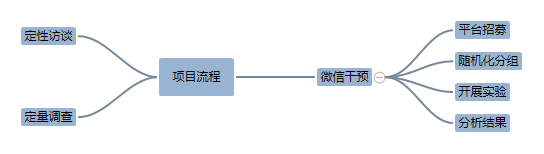
\includegraphics[width=\textwidth]{newprocess.png}
	\centering
	\caption{项目设计简图}
\end{figure}